\documentclass{article}

% Language setting
% Replace `english' with e.g. `spanish' to change the document language
\usepackage[english]{babel}

% Set page size and margins
% Replace `letterpaper' with `a4paper' for UK/EU standard size
\usepackage[a4paper,top=2cm,bottom=2cm,left=2cm,right=2cm,marginparwidth=1.5cm]{geometry}

\usepackage{chngcntr}

\counterwithin*{section}{part} % Resets section counter after every part
\renewcommand{\thesection}{Ex \arabic{section}.} % Prefixing section numbers with "Ex"
\setcounter{section}{-1} % Starting section count from -1 so that it begins with "Ex 0."

% Useful packages
\usepackage{amsmath}
\usepackage{graphicx}
\usepackage{subcaption}
\usepackage[colorlinks=true, allcolors=blue]{hyperref}

\usepackage[product-units = power]{siunitx}
\sisetup{round-precision=2, separate-uncertainty = true, detect-weight=true, detect-family=true}
\usepackage[capitalise,nameinlink]{cleveref}
\usepackage{physics}
\AtBeginDocument{\RenewCommandCopy\qty\SI}
\usepackage[version=4]{mhchem}

\usepackage{booktabs}
\usepackage{multirow}

\title{MP2\\Path Integration using Coupled Bump Attractors\\---\\Computational neurosciences: neuronal dynamics\\NX-465}
\author{Konstantin Weindel}

\begin{document}
\maketitle


\section*{Introduction}
In this mini project 

\section{Getting Started: Poisson neurons}
\subsection*{0.1.}
\begin{figure}[h]
    \centering
    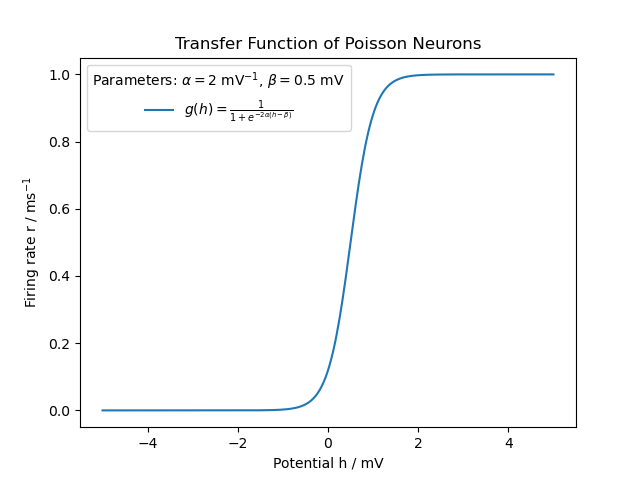
\includegraphics[width=0.5\textwidth]{figures/0.1.transfer_function.png}
    \caption{For Poisson Neurons, firing rate \(r\) in dependence of the potential \(h\) is described by a sigmoid function with parameters \(\alpha\) and \(\beta\).}
    \label{fig:01}
\end{figure}

The firing rate \(r_i\) of a Poisson Neuron \(i\) in dependence of it's potential \(h_i\) can be described by the in \cref{fig:01} depicted transfer function:
\[g(h_i(t)) = \frac{1}{1+\exp{-2\alpha(h_i(t)-\beta)}}.\]
The parameter $\alpha$ determines the steepness of the curve. A higher value of $\alpha$ makes the transition from the low firing rate to the high firing rate more abrupt.
The parameter $\beta$ sets the threshold potential at which the firing rate increases significantly. If $h_i(t)$ is much less than $\beta$, the firing rate $r_i(t)$ will be close to 0. If $h_i(t)$ is much greater than $\beta$, the firing rate will approach $r_0$.

\subsection*{0.2.}
\begin{table}[h]
\centering
\begin{tabular}{@{}rcc@{}}
\toprule
N    & mean number of spikes / \unit{\per\milli\second} & instantaneous rate r / \unit{\per\milli\second} \\ \midrule
100  &0.1173099& \multirow{2}{*}{0.1192043}                                                                                    \\
1000 &0.118458&                                                                                                               \\ \bottomrule
\end{tabular}
\caption{The number of spikes for a set of \(N\) neurons are calculated stochastically and analytically.}
\label{tab:02}
\end{table}

\Cref{tab:02} shows the result of the firing dynamics of unconnected neurons.
The mean number of spikes per ms across the N neurons differs from the instantaneous rate due to the stochastic nature of spike generation in the Poisson process. The actual spike count can vary around the expected value given by the rate equation.
With a larger number of neurons, the law of large numbers suggests that the mean spike count should more closely approximate the expected rate (instantaneous rate), reducing the variability seen in the smaller population.

\section{Bump attractor}
\subsection*{1.1.}\label{sec:11}
\begin{figure}[h!]
  \centering
  \begin{subfigure}[b]{0.32\textwidth}
    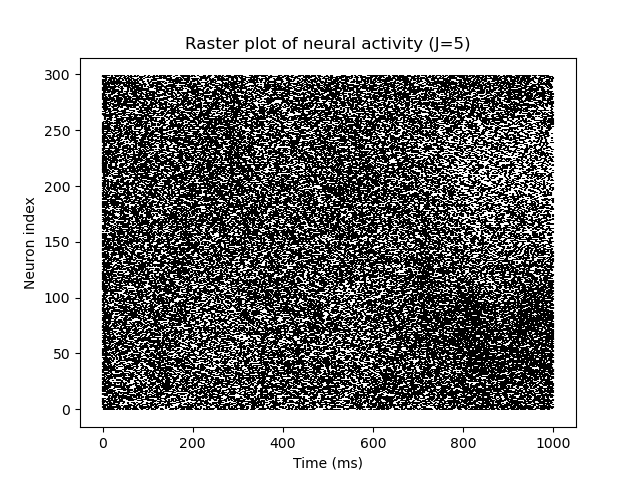
\includegraphics[width=\textwidth]{figures/1.1.raster_plot_J5.png}
    \caption{\(J=\qty{5}{\pico\coulomb}\).}
    \label{fig:J5}
  \end{subfigure}
  \hfill
  \begin{subfigure}[b]{0.32\textwidth}
    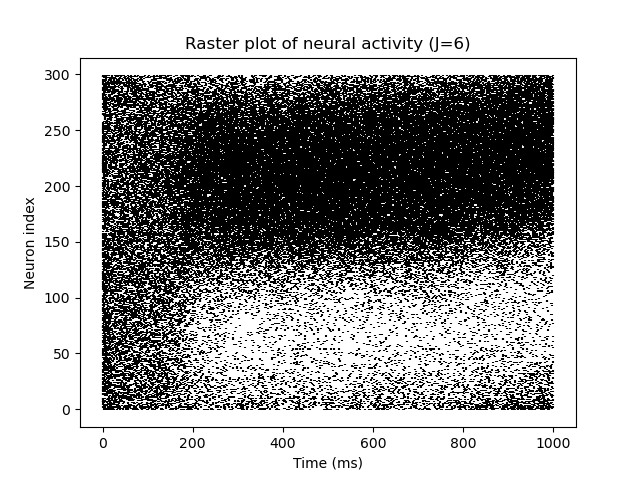
\includegraphics[width=\textwidth]{figures/1.1.raster_plot_J6.png}
    \caption{\(J=\qty{6}{\pico\coulomb}\).}
    \label{fig:J6}
  \end{subfigure}
  \hfill
  \begin{subfigure}[b]{0.32\textwidth}
    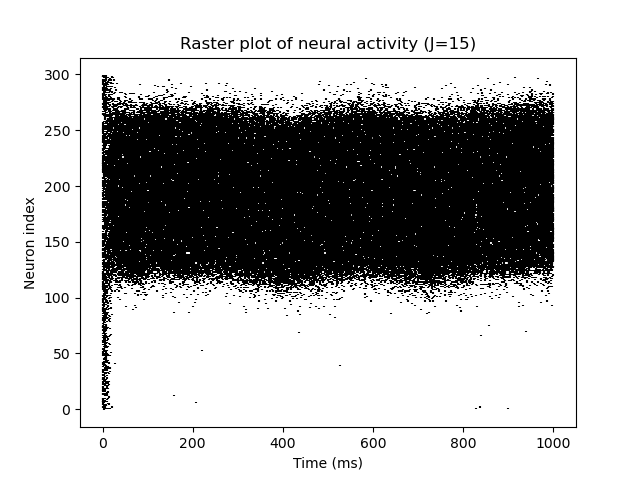
\includegraphics[width=\textwidth]{figures/1.1.raster_plot_J15.png}
    \caption{\(J=\qty{15}{\pico\coulomb}\).}
    \label{fig:J15}
  \end{subfigure}
  \caption{The dynamics of a recurrent network with no external input with varying degrees of interaction strength \(J\).}
  \label{fig:J}
\end{figure}

For a recurrent network with \(N=300\) neurons the dynamics for different interaction strengths \(J\) are shown in the raster plots in \cref{fig:J}. With increasing interaction strength \(J\) a more and more stable bump is attracted and maintained in the network. In the given setup, stability can be assumed from \(J>\qty{9}{\pico\coulomb}\).

\subsection*{1.2.}
\begin{figure}[h]
    \centering
    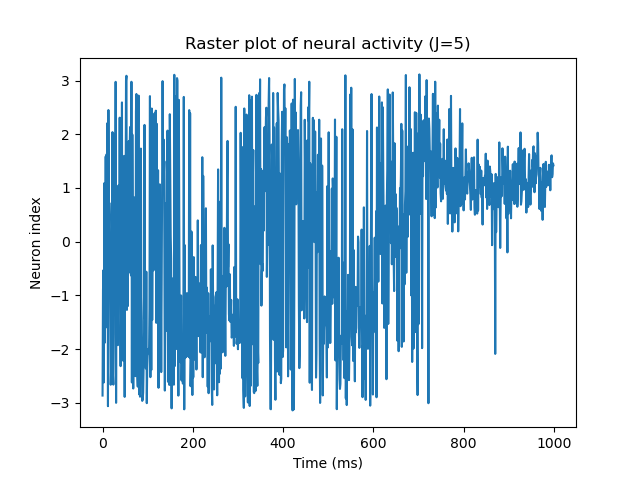
\includegraphics[width=0.5\textwidth]{figures/1.2.stability_plot_J5.png}
    \caption{The location of the bump \(\theta_\text{bump}\) in a recurrent network with \(J=\qty{5}{\pico\coulomb}\) shows drift effects while having more stable phases in between.}
    \label{fig:11}
\end{figure}
The location of the bump \(\theta_\text{bump}\) over time, shown in \cref{fig:11}, is found using a weighted version of the circular mean.

\subsection*{1.3.}
The location of the bump can drift due to the inherent stochasticity in the firing of Poisson neurons. Since the spikes are generated according to a Poisson process, there is randomness in the timing of each neuron's firing. This randomness can cause fluctuations in the collective activity, leading to the drift of the bump's location over time.

To improve the stability of the bump and reduce drift, the parameters of the model could be modified in the following ways:
\begin{itemize}
    \item Increase the Number of Neurons (\(N\)): A larger number of neurons can average out the randomness and reduce fluctuations, leading to a more stable bump. With more neurons, the effects of random spikes are less pronounced on the overall activity pattern.
    \item Increase the time constant (\(\tau\)): A larger time constant can smooth the fluctuations in the activity, as the potential decays more slowly. While potentially increasing the stability, this might reduce the network's response to changes.
    \item Decrease the time step (\(\Delta t\)): A smaller time step can improve the qualitiy of the numerical integration, capturing the dynamics of the network more precisely and potentially reducing drift.
    \item Interaction Strength (\(J\)): As shown in \cref{sec:11} the choice of \(J\) plays a role on the stability of the bump.
    \item Transfer Function Parameters (\(\alpha\),\(\beta\)): The shape of the transfer function influences the neuron's responsiveness to input and can therefore also be used to adjust for stability.
\end{itemize}

\subsection*{1.4.}
\begin{figure}[h]
    \centering
    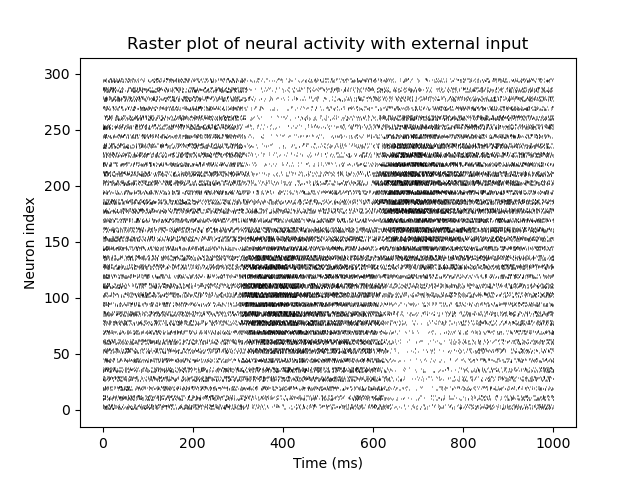
\includegraphics[width=0.5\textwidth]{figures/1.4.extinput_plot_J5.png}
    \caption{Raster plot of the spikes of the recurrent network from above, now driven with an external input.}
    \label{fig:14}
\end{figure}

The external current is defined as a Gaussian function centered at two different locations, \( \mu^{(1)} \) and \( \mu^{(2)} \), with a standard deviation \( \sigma \).
The effect of this input on the bump can be observed in the raster plot in \cref{fig:14}. Typically, the external current will cause the bump to shift towards the location of the current. This happens because the neurons at the location of the current receive additional input, increasing their firing rate and attracting the bump.
The connectivity profile, which is based on the cosine of the difference in positions, supports this behavior. Neurons that are closer in position have stronger connections (higher cosine values), so when a group of neurons receives an external current, it can influence its neighbors more strongly than distant neurons. This localized increase in activity can pull the bump towards the current's location.

\subsection*{1.5.}
\begin{figure}[h]
    \centering
    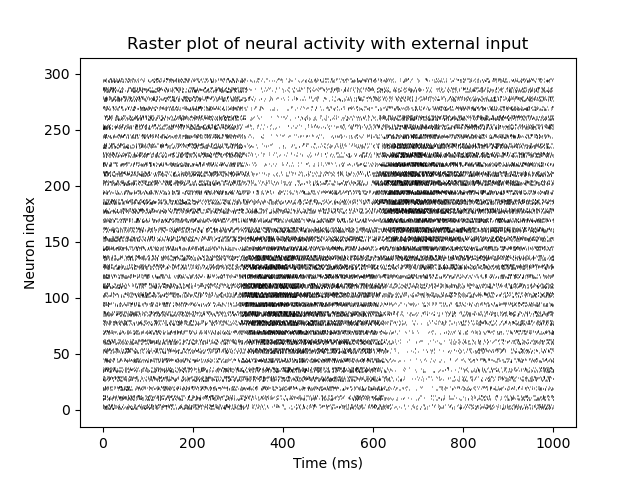
\includegraphics[width=0.5\textwidth]{figures/1.4.extinput_plot_J5.png}
    \caption{Raster plot of the spikes of the recurrent network from above, now driven with an external input.}
    \label{fig:14}
\end{figure}

If the connectivity in the network is given by \( w(x_i - \varphi, x_j) \), where \( \varphi \) is a small angle, this would introduce a phase shift in the interactions between neurons. The connectivity would no longer be symmetric around zero, and this asymmetry would cause the bump to drift in the direction of the phase shift.



\section{Integration}

\section{Path integration}
\subsection{}
To generate the random trajectory in two dimensions, I used a vector to describe the position of each dimension in the Cartesian plane ($x$ and $y$). I then chose a fixed starting position (since this is arbitrary and can be transformed to any starting position) as the point $[0,0]$.
At each time point a random future direction (the heading, $\theta$) is drawn from a uniform distribution and the cosine and sine of the heading is used to change $x$ and $y$ values respectively based on the previous values and a step size $S$: 
\begin{equation*}
    x{t} = x_{t - 1} S cos(\theta_{t})
\end{equation*}
\begin{equation}
    y{t} = y_{t - 1} S sin(\theta_{t})
\end{equation}

\begin{figure}
    \centering
    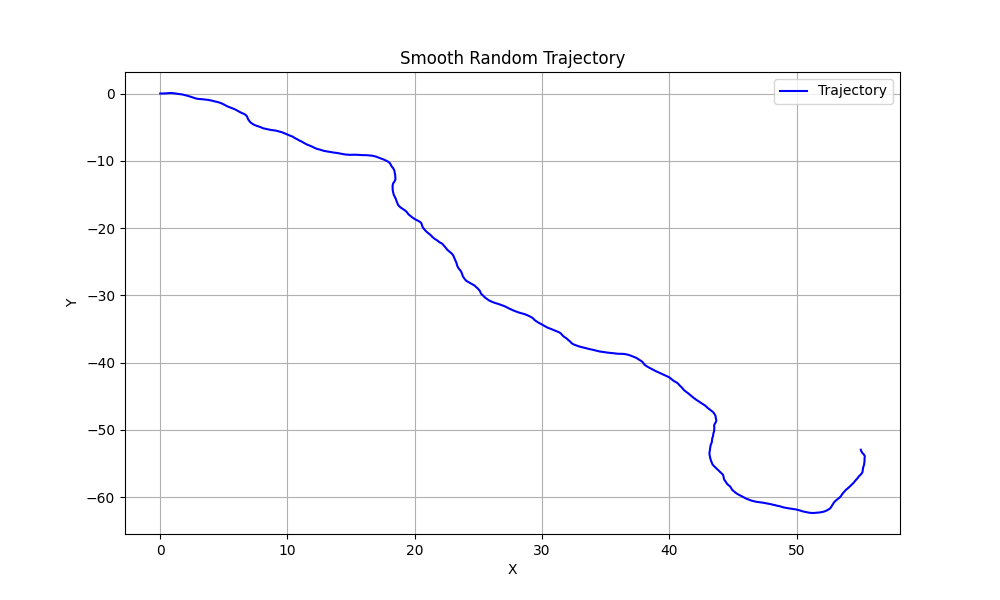
\includegraphics[width=0.6\textwidth]{konsta_31.png}
    \caption{Caption}
    \label{fig:enter-label}
\end{figure}


\end{document}